\chapter{Experimentos e resultados}
\label{cap:resultados}

Este capítulo apresenta os resultados obtidos com os procedimentos descritos
no \autoref{cap:metodos}, na máquina de referência
(Tabela~\ref{tab:ambiente}), na execução de referência de 10 de setembro de
2026. Todos os números são oriundos de execução real e podem ser reproduzidos
pelos comandos descritos no \autoref{ap:repositorio}.

\section{Verificação funcional automatizada}
\label{sec:res_testes}

A suíte automatizada cobre as seis etapas do desenvolvimento e o adaptador de
IA. A Tabela~\ref{tab:testes} detalha a distribuição das verificações por
etapa; a Figura~\ref{fig:verificacoes} apresenta a mesma informação
visualmente. No total, foram executadas \textbf{211 verificações do motor e 16
testes do adaptador, todas aprovadas}, sem falhas.

% Verificações automatizadas por etapa (capítulo 6).
\begin{table}[htbp]
\centering
\caption{Verificações automatizadas por etapa do projeto (execução de referência de 2026-09-10).}
\label{tab:testes}
\footnotesize
\begin{tabular}{@{}>{\raggedright\arraybackslash}p{1.6cm} >{\raggedright\arraybackslash}p{8.4cm} >{\centering\arraybackslash}p{2.2cm}@{}}
\toprule
Etapa & Escopo validado & Verificações \\
\midrule
\poc{1} & Fundação jogável: entrada semântica, movimento, colisão, câmera, pausa, HUD e diagnóstico de entrada & 77 \\
\poc{2} & Laboratório funcional: interação, inventário, porta, missão, identidade visual da sala & 34 \\
\poc{3} & IA: adaptador, terminal, limites de tempo, validação de intenção e \emph{fallback} & 25--26 \\
\poc{4} & Mundo reativo: NPC, luzes por energia, câmera de segurança, tom da IA e memória em camadas & 21 \\
\poc{5} & Laboratório procedural: determinismo por semente e conectividade entre módulos & 23 \\
\poc{6} & Recorte vertical: tutorial, missão completa, persistência, áudio e epílogo & 30 \\
Adaptador & API de IA (Python): contratos, validação, erros e limites & 16 \\
\midrule
\textbf{Total} & & \textbf{211 + 16} \\
\bottomrule
\end{tabular}
\par\vspace{2pt}{\footnotesize Fonte: elaborado pelo autor (2026), a partir da execução de \texttt{tests/run\_all.sh}. A etapa \poc{3} vale 25 com o adaptador no ar e 26 com o adaptador desligado.}
\end{table}


\begin{figure}[htbp]
\centering
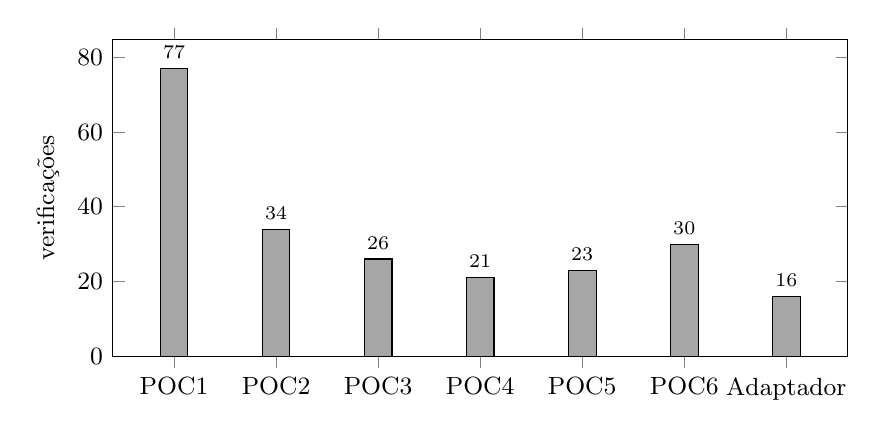
\begin{tikzpicture}
\begin{axis}[
  ybar,
  width=0.9\textwidth,
  height=5.6cm,
  bar width=10pt,
  ymin=0,
  ylabel={verificações},
  symbolic x coords={POC1,POC2,POC3,POC4,POC5,POC6,Adaptador},
  xtick=data,
  nodes near coords,
  every node near coord/.append style={font=\scriptsize},
  tick label style={font=\small},
  label style={font=\small},
]
\addplot[fill=black!35] coordinates {
  (POC1,77) (POC2,34) (POC3,26) (POC4,21) (POC5,23) (POC6,30) (Adaptador,16)
};
\end{axis}
\end{tikzpicture}
\caption{Distribuição das verificações automatizadas por etapa do projeto, incluindo os testes do adaptador de IA.}
\label{fig:verificacoes}
\par\vspace{2pt}{\footnotesize Fonte: elaborado pelo autor (2026), a partir da execução da suíte.}
\end{figure}

Dois comentários sobre a leitura da tabela. Primeiro, a etapa \poc{3} varia
entre 25 e 26 verificações: com o adaptador no ar, um dos casos de
\emph{fallback} dá lugar à validação da resposta real do modelo, de modo que
o número depende do contexto de execução. Segundo, o tamanho da suíte não é
uniforme entre etapas --- a fundação jogável concentra 77 verificações porque
precisou cobrir movimento, colisão, câmera, entrada e interface.

\section{Critérios de aceitação}
\label{sec:res_criterios}

A Tabela~\ref{tab:aceitacao_resumo} resume o status dos critérios de
aceitação. Treze dos quatorze itens verificáveis são cobertos por testes
automatizados; os pontos de contato físico (mouse capturado e joystick real)
e o percurso completo por uma pessoa permanecem como validação manual
declarada. O requisito de empacotamento (FR-033) segue aberto: a geração do
executável dependia de modelos de exportação do motor ausentes no ambiente.

% Status dos critérios de aceitação (capítulo 6).
\begin{table}[htbp]
\centering
\caption{Status dos critérios de aceitação e requisito de empacotamento.}
\label{tab:aceitacao_resumo}
\footnotesize
\begin{tabular}{@{}>{\raggedright\arraybackslash}p{1.5cm} >{\raggedright\arraybackslash}p{8.0cm} >{\raggedright\arraybackslash}p{2.6cm}@{}}
\toprule
Critério & Verificação & Status \\
\midrule
CA-001 & Movimento por ação semântica, colisão e piso & Aprovado (automatizado) \\
CA-002 & Rotação de câmera por ação; limites de inclinação & Parcial (mouse = manual) \\
CA-003 & Pausa e retomada com menu & Aprovado (automatizado) \\
CA-004 & Zona morta configurável e tratamento de \emph{hotplug} & Parcial (joystick físico = manual) \\
CA-005 & Carga do jogo sem assets externos obrigatórios & Aprovado (automatizado) \\
CA-006 & Convite contextual e interação por proximidade & Aprovado (automatizado) \\
CA-007 & Coleta, instalação no painel e avanço da missão no HUD & Aprovado (automatizado) \\
CA-008 & Estados de equipamento serializáveis (desligado, falha, pronto, operando) & Aprovado (automatizado) \\
CA-009 & \emph{Fallback} com o serviço de IA indisponível, sem travar & Aprovado (automatizado) \\
CA-010 & Intenção fora do conjunto permitido convertida para \texttt{NONE} & Aprovado (automatizado) \\
CA-011 & Mundo reage a eventos (NPC, luzes, tom da IA) & Aprovado (automatizado) \\
CA-012 & Mesma semente produz o mesmo layout; salas alcançáveis & Aprovado (automatizado, 6 sementes) \\
CA-013 & Jogo completo do início ao fim & Parcial (percurso humano = manual) \\
FR-033 & Geração de executável independente & Aberto (modelos de exportação ausentes no ambiente) \\
\bottomrule
\end{tabular}
\par\vspace{2pt}{\footnotesize Fonte: elaborado pelo autor (2026), a partir da especificação e da execução da suíte.}
\end{table}


\section{Desempenho gráfico}
\label{sec:res_desempenho}

A cena completa --- com a sala detalhada, o NPC, as camadas de iluminação e
os letreiros --- executou a \textbf{60 quadros por segundo}, limitados por
sincronismo vertical, em resolução de 1280$\times$720, na GPU integrada AMD
Radeon Graphics. O valor foi mantido após o detalhamento final da sala (342
nós e 37 materiais no asset), dentro do critério NFR-001. A
Figura~\ref{fig:sala_energizada} mostra a cena com a energia restabelecida ---
o estado em que sensores, luzes e câmera de segurança estão todos ativos, ou
seja, o cenário mais carregado do jogo.

\begin{figure}[htbp]
\centering

\includegraphics[width=0.8\textwidth]{sala_energizada.png}
\caption{Sala com a energia restaurada: luminárias do teto acesas, câmera de segurança ativa, porta B1 liberada e letreiros das estações. Captura em 1280$\times$720.}
\label{fig:sala_energizada}
\end{figure}

Duas ressalvas tornam a leitura honesta. A primeira: o valor de 60 quadros
por segundo é um limite imposto pelo sincronismo vertical, não uma medida de
folga do sistema; sem sincronismo, a taxa observada seria maior, mas o
trabalho não mediu esses valores. A segunda: não foram coletadas métricas de
tempo de quadro por percentil (por exemplo, o quadro mais lento de cada
segundo), que seriam necessárias para caracterizar engasgos transitórios
[MEDIÇÃO DE FRAME TIME NÃO REALIZADA]. Ambas as lacunas estão registradas
como trabalhos futuros.

\section{Complexidade do asset 3D}
\label{sec:res_asset}

A inspeção programática do arquivo exportado mediu: 342 nós, 37 materiais,
35 nós de colisão embutidos e tamanho final de 1.018,7~KB. Esses números
delimitam o orçamento de complexidade do cenário e explicam, em parte, o
desempenho obtido: o detalhamento foi feito com geometria econômica e
materiais reutilizados, e as animações que o formato não suporta (emissão
intermitente) foram convertidas em lógica de script.

\section{Latência da conversa com a IA}
\label{sec:res_latencia}

A Tabela~\ref{tab:latencia} apresenta as três medições de latência
realizadas com o modelo local \texttt{llama3.1:8b}. O pior caso (22,0~s) foi
a chamada direta ao adaptador em partida fria, quando o modelo precisa ser
carregado na memória; no uso cotidiano pelo terminal do jogo, a resposta
levou 16,1~s; e no teste ao vivo do cliente, 12,9~s, com aprovação integral
das verificações de integração.

% Latências medidas (capítulo 6).
\begin{table}[htbp]
\centering
\caption{Latências medidas da conversa com a IA local (\texttt{llama3.1:8b}) em três contextos independentes.}
\label{tab:latencia}
\footnotesize
\begin{tabular}{@{}>{\raggedright\arraybackslash}p{5.4cm} l r >{\raggedright\arraybackslash}p{3.4cm}@{}}
\toprule
Contexto & Intenção & Latência & Observação \\
\midrule
Chamada direta ao adaptador (partida fria) & DIAGNOSE & 22,0 s & confiança 0,9 \\
Terminal no jogo (uso normal) & STATUS & 16,1 s & evidência visual capturada \\
Cliente no jogo (teste ao vivo) & HINT & 12,9 s & 5 de 5 verificações \\
\bottomrule
\end{tabular}
\par\vspace{2pt}{\footnotesize Fonte: elaborado pelo autor (2026). Uma execução por contexto; valores indicativos, não estatísticos.}
\end{table}


A Figura~\ref{fig:terminal_evidencia} registra a evidência visual do
contexto em jogo: a pergunta do jogador e a resposta do modelo, exibidas no
terminal da \aria{}. A Figura~\ref{fig:tela_evidencia} mostra a tela de status
da estação no mundo 3D, que dá coerência diegética ao subsistema.

\begin{figure}[htbp]
\centering

\includegraphics[width=0.8\textwidth]{terminal_aria.png}
\caption{Terminal da \aria{} no jogo com a resposta do modelo local (latência de 16,1~s, intenção \texttt{STATUS}).}
\label{fig:terminal_evidencia}
\end{figure}

\begin{figure}[htbp]
\centering

\includegraphics[width=0.8\textwidth]{tela_aria.png}
\caption{Tela de status da estação da IA no mundo 3D, com identificação do núcleo e do canal de comunicação.}
\label{fig:tela_evidencia}
\end{figure}

Três observações qualificam esses números. Primeiro, as medições foram feitas
com um modelo \emph{maior} do que o alvo declarado no projeto
(\texttt{llama3.2:3b}, não instalado no ambiente): espera-se que o modelo-alvo
seja mais rápido, mas isso não foi medido [MODELO-ALVO NÃO EXECUTADO].
Segundo, cada contexto foi medido em uma execução; os valores são
indicativos, não estatísticos. Terceiro, o comportamento de segurança foi
verificado independentemente das medições de velocidade: com o serviço fora
do ar, o jogo respondeu com texto de \emph{fallback} e intenção \texttt{NONE},
sem travar --- resultado coberto pelos testes automatizados do adaptador e do
cliente.

\section{Evidências visuais e demonstração}
\label{sec:res_evidencias}

Além das figuras deste capítulo, o projeto mantém um conjunto de evidências
visuais produzido por um arnês de captura que posiciona o jogador em pontos
pré-determinados, podendo inclusive concluir a missão para registrar o estado
final (a Figura~\ref{fig:sala_energizada} foi gerada nesse modo). Um vídeo de
demonstração de 1~min~08~s percorre a missão do segundo incremento, do painel
à abertura da porta \cite{lab404video}. Código, especificação, capturas e
vídeo estão publicamente disponíveis \cite{lab404repo}.

\section{Reprodutibilidade dos resultados}
\label{sec:reprodutibilidade}

Todos os resultados deste capítulo são reproduzíveis a partir do repositório
público \cite{lab404repo} com os comandos a seguir; na primeira execução, o
projeto importa os recursos (modelo 3D e áudio), e nas seguintes os comandos
abaixo bastam.

\begin{itemize}
  \item \texttt{tests/run\_all.sh} --- executa a suíte completa e imprime, por
  etapa, o número de verificações e de falhas (esperado: todas aprovadas);
  \item \texttt{godot4 --path .} ou \texttt{./start.sh} --- inicia o jogo (o
  segundo inicia também o serviço de IA, quando o ambiente Python existe);
  \item \texttt{.venv/bin/uvicorn scripts.aria\_adapter:app --port 8000} ---
  inicia o serviço de IA, com o modelo local servido pelo Ollama;
  \item cena de captura com variáveis de pose e de conclusão da missão ---
  reproduz as imagens de evidência deste capítulo;
  \item script de inspeção do arquivo GLB --- reproduz as contagens de nós,
  materiais e colisões.
\end{itemize}

Variações de hardware, de versão de biblioteca e de modelo de linguagem
alteram os valores de desempenho e de latência, mas não os resultados
funcionais: a suíte é determinística no que verifica, e a geração procedural
é determinística por semente.

\section{Matriz de evidências}
\label{sec:res_matriz}

O Quadro~\ref{quad:matriz} resume a correspondência entre as afirmações
quantitativas do trabalho e as evidências que as sustentam --- a versão
completa está no arquivo de rastreabilidade do projeto.

\begin{quadro}[htbp]
\centering
\caption{Correspondência entre afirmações quantitativas e evidências.}
\label{quad:matriz}
\footnotesize
\begin{tabular}{@{}>{\raggedright\arraybackslash}p{4.6cm} >{\raggedright\arraybackslash}p{4.4cm} >{\raggedright\arraybackslash}p{3.8cm}@{}}
\toprule
Afirmação & Evidência & Fonte \\
\midrule
211 verificações do motor + 16 testes do adaptador aprovados & Execução da suíte completa & \texttt{tests/run\_all.sh}; cenas de teste e suíte Python \\
60 FPS (vsync) em 1280$\times$720 na GPU integrada & Leitura do motor em execução na cena completa & Execução na máquina de referência (Tabela~\ref{tab:ambiente}) \\
Latências de 12,9 s a 22,0 s & Três execuções cronometradas & Relatório de execução e captura do terminal \\
342 nós, 37 materiais, 35 colisões, 1.018,7 KB & Inspeção programática do GLB & \texttt{assets/lab404/}\allowbreak\texttt{lab\_sala\_poc2.glb} \\
Missão completa do início ao fim (automatizado) & Cena de teste da etapa final & \texttt{tests/poc6\_test.gd} \\
Degradação segura da IA sob falha & Testes de contrato e de integração & CA-009 e CA-010 (suíte do adaptador) \\
\bottomrule
\end{tabular}
\par\vspace{2pt}{\footnotesize Fonte: elaborado pelo autor (2026).}
\end{quadro}

\section{Síntese dos resultados}
\label{sec:res_sintese}

Em síntese, os experimentos demonstram: (i) o sistema é funcionalmente
verificável --- 227 verificações automatizadas no total, todas aprovadas;
(ii) o desempenho atende ao critério de hardware modesto no cenário mais
carregado; (iii) a integração com a IA local funciona de ponta a ponta, com
latências de 12,9~s a 22,0~s e degradação segura garantida; e (iv) o
artefato 3D permanece dentro de um orçamento de complexidade compatível com
GPU integrada. As limitações desses resultados --- e o que elas implicam ---
são discutidas no capítulo seguinte.
